In this section the conformation of FAK bound to a \pip{} containing membrane (FAK-MEM) is compared to the observations of FAK-SOL. To this end FAK structures of setup 4 were used with the condition that the FAK molecules have no neighbours. The contact map is based on the same dataset, which was used for \autoref{force:contactmap}.\\
\\
Regarding $d_\text{F2-C}$ a closure of F2 and the C-lobe can be obtained. Large values up to $3.8\,\si{\nano\metre}$, such as in spot 1 of FAK-SOL, disappear (\autoref{mem:comdist}). Since both, FERM domain and kinase, have a docking site for \pip{} which binds them to the membrane, this stabilisation is reasonable. In contrast the distribution of $d_\text{F2-C}$ induces that a partial opening of the interface between F1 and the N-lobe gets more preferred. As explained in \autoref{sec:fak_sol} the linker is located in this region for FAK-SOL.\\
The closure of F2 and the C-lobe influences the contact area as well. In comparison to FAK-SOL, it is increased to $30.8\,\si{\nano\metre}^2$ (\autoref{mem:contactarea}).\\
\\
A more detailed insight can be obtained from the contact map. For an easier comparison, the difference between the contact map of FAK-SOL and FAK-MEM is shown in \autoref{mem:contact}. At the interface of F2 and the C-lobe (area 1) the residue distances get closer, which is consistent with the decreasing $d_\text{F2-C}$. In area 2 both, increasing and decreasing distances can be found. Regarding the 3D structure one can see that the residues of the FERM domain, which get closer to the kinase, are located nearer to F2 than those getting farther away. In addition all residues of the FERM domain getting farther away from residues \acid{S}{574} to \acid{A}{579} of the kinase, which also include the activity regulating residues \acid{Y}{576} and \acid{Y}{577}.\\
Also in the linker region conformational changes can be observed. Area 3 indicates that the ball structure of the \acid{Y}{397} containing ball structure observed in FAK-SOL disappears. As shown in \autoref{3D} the residues unravel and cling to the FERM domain. By this the autophosphorylation site \acid{Y}{397} gets more exposed.\\
\\
As suggested by experimental results the FERM domain does not dissociate from the kinase because of binding to \pip{}. However this binding leads to conformational changes resulting in a partial opening of the FERM kinase interface and the exposure of the autophosphorylation site \acid{Y}{397} \autocites{pap001}{pap003}.
%
%
%
\begin{figure}
	\subcaptionbox{\label{mem:comdist}}[0.49\textwidth]{
		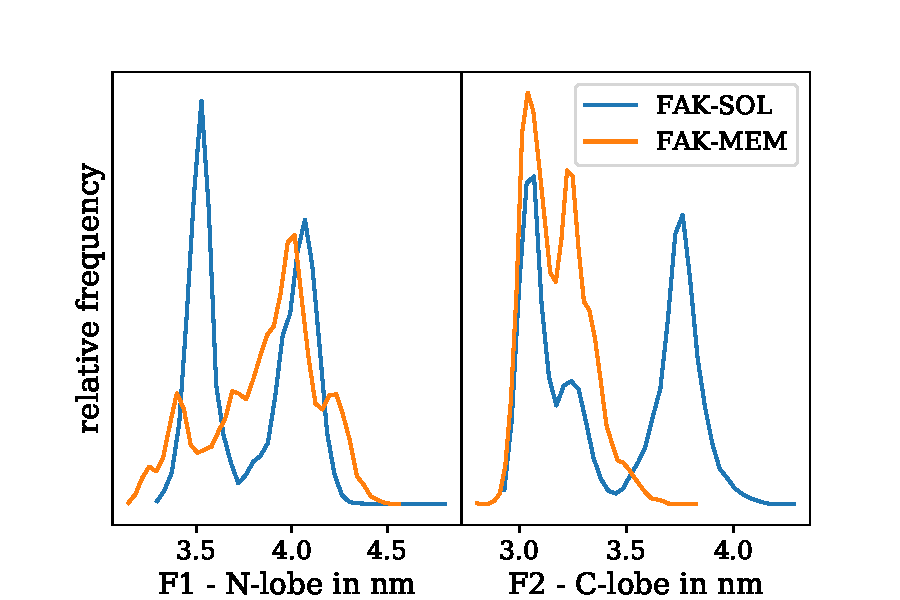
\includegraphics[height=5cm]{figures/results/comp_free_mem_comdist}
	}\hfill%
	\subcaptionbox{\label{mem:contactarea}}[0.49\textwidth]{
		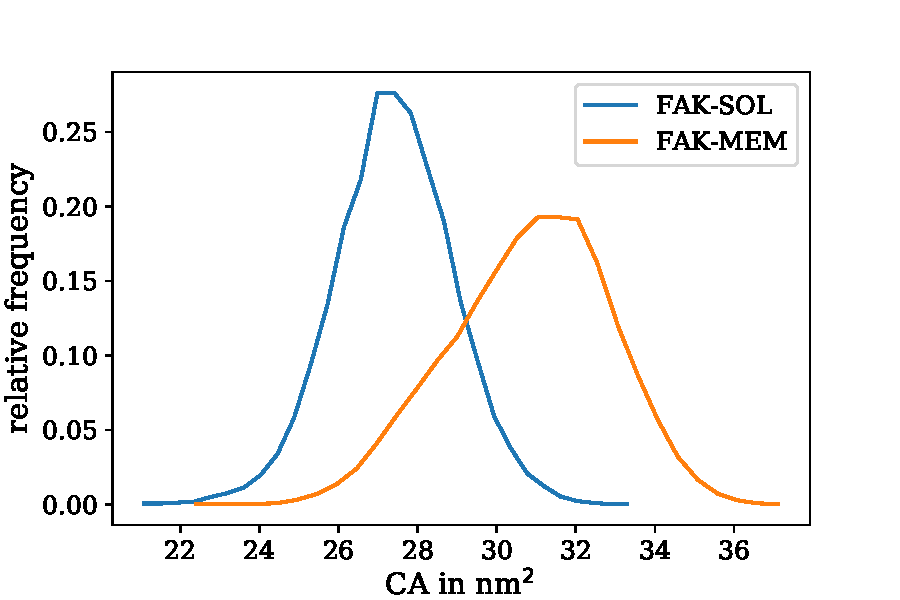
\includegraphics[height=5cm]{figures/results/ca_sol_mem}
	}%
	\nicecaption{Domain distances and contact area of FAK-MEM}{(\subref{mem:comdist}): distribution of $d_\text{F1-N}$ and $d_\text{F2-C}$ in comparison to FAK-SOL. (\subref{mem:contactarea}): contact area in comparison to FAK-SOL}
\end{figure}
%
%
%
%
%
%
\begin{figure}
	\centering
	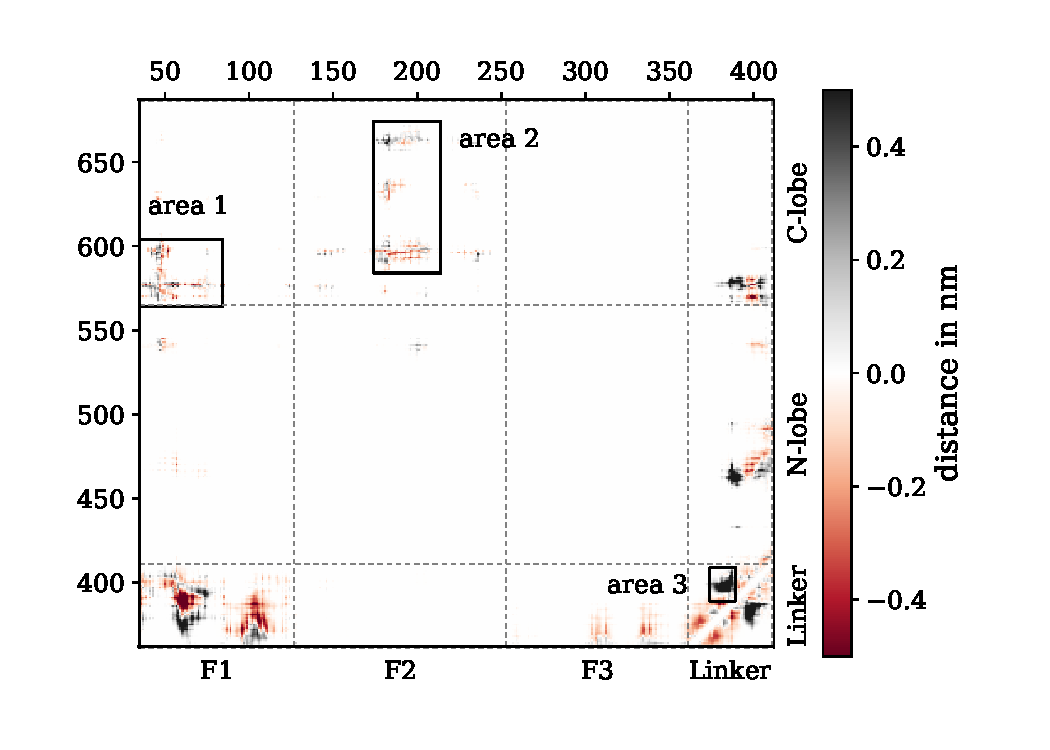
\includegraphics[width=.8\textwidth]{figures/results/contactmap_diff_to_free}
	\nicecaption{Difference contact map of FAK-MEM}{The contact map shows the difference FAK-MEM - FAK-SOL in the distances.}
	\label{mem:contact}
\end{figure}
%
%
%
